\newif\ifPDF
\ifx\pdfoutput\undefined\PDFfalse \else\ifnum\pdfoutput >
0\PDFtrue
    \else\PDFfalse
    \fi
\fi

\documentclass[a4paper,11pt,openany,notitlepage]{article}

\title{
\begin{flushright}
Development of an OMGeo Open Markup Format \\ {for the Open GIS Consortium Web Map Service}
\\ {\large{320342 - Guided Research Computer Science -}} \\ {\normalsize{Project Proposal}}
\end{flushright}}
\author{}
\date{}

\usepackage{fancyhdr}
\usepackage{bm}
\usepackage{../../../doc/macros/draftstamp}

\linespread{1.0}

\ifPDF
\usepackage[pdftex]{color,graphicx}
\usepackage[pdftex,bookmarks=true]{hyperref}
\else
\usepackage[dvips]{graphicx}
\usepackage[dvips,bookmarks=true]{hyperref}
\fi

\pagestyle{fancy}
% with this we ensure that the chapter and section
% headings are in lowercase.
%\renewcommand{\chaptermark}[1]{\markboth{#1}{}}
\renewcommand{\sectionmark}[1]{\markright{\thesection\ #1}}
\fancyhf{} % delete current setting for header and footer
\fancyhead[R]{\bfseries\thepage}
\fancyhead[L]{\bfseries\rightmark}
\renewcommand{\headrulewidth}{0.5pt}
\renewcommand{\footrulewidth}{0pt}
\addtolength{\headheight}{2.5pt} % make space for the rule
\addtolength{\textwidth}{1.5cm} \addtolength{\headwidth}{1.5cm}
\addtolength{\topmargin}{-1.0cm} \addtolength{\textheight}{2.2cm}
\addtolength{\hoffset}{-0.5cm}
\fancypagestyle{plain}{%
    \fancyhead{} % get rid of headers on plain pages
    \renewcommand{\headrulewidth}{0pt} % and the line
}

\hypersetup{colorlinks,%
    linkcolor=blue,%
    citecolor=blue,%
    filecolor=blue,%
    urlcolor=blue,%
    bookmarksnumbered,
    bookmarksopen,%
    pdfstartview=FitV,%
    plainpages=false,%
    hypertexnames=false,%
    a4paper}

%%%%%%%%%%%%%%%%%%%%%%%%%%%%%%%%%%%%%%%%%    
\begin{document}

\pagenumbering{roman}
\maketitle \hrule
\begin{flushright}
\Large{\textbf{Alexandru A. Chitea}}
\end{flushright}

\begin{flushright}
\small{a.chitea@iu-bremen.de}
\end{flushright}
\vspace{1cm}
\begin{flushright}
\large{Project Coordinators:}
\end{flushright}

\begin{flushright}
\normalsize{Dr. Peter Baumann - p.baumann@iu-bremen.de}
\end{flushright}
\begin{flushright}
\normalsize{Dr. Michael Kohlhase - m.kohlhase@iu-bremen.de}
\end{flushright}
\vspace{11cm}
International University Bremen\hspace{1.25cm} March 7, 2005\hspace{1.25cm} Spring Semester 2005


\newpage
\tableofcontents
\listoffigures % comment out if you have no figures
\listoftables  % comment out if you have no tables
\pagenumbering{arabic}
\newpage
\section{Executive Summary} \label{sec:execsummary}
\indent

Web Map Services\footnote{The proposed project refers to the Open GIS Consortium WMS Implementation Specification (version 1.1.1) \cite{ogc}.} (WMSes) have been successfully used in a broad range of applications, from meteorology to disaster mitigation. Moreover, as academic and research tools, they are employed by geoscientists to explore discrete properties of the Earth's surface, such as, for example, elevation levels or marine shorelines.

As the WMSes in use today are targeted to specific application areas and cultural backgrounds, their application programming interfaces (APIs) and user-interfaces are therefore hard-coded accordingly. However, most of the times geodata maps need to be exchanged between several clients or manipulated by software applications. A good illustration is the interpretation of two national roadmaps for navigation purposes. For example, when using the German Brandenburg WMS\footnote{The service is restricted to academic use, and hence we cannot provide a valid access URL.}, the term \textit{Strassenorange}\footnote{\textit{Strassenorange} stands for orange street in German.} represents a small road, whereas a French WMS might encode the same data with a different keyword. Therefore the combination of visual representation and the geodata itself leads to conflicts\footnote{E.g.,the language and abbreviated terms may not be international.} between data function and its format, creating bottlenecks in terms of usability.

So far, various schemes for georeferenced data representation have been developed at national scales, but none has yet been adopted as an international standard. The proposed project aims at separating data appearance from its structure through a semantic-based and context-aware technique \cite{mkm2005}. As the OMDoc (\textit{Open Mathematical Documents}) format \cite{kohlhase2004} represents an established method for mathematical knowledge representation and management, we consider extending it to encompass geosemantics. If we succeed in our endeavor, we will achieve a high degree of flexibility in terms of geodata manipulation. Among many others, an envisioned area of application is the disaster mitigation public services\footnote{As major natural cataclysms usually span more than one country, it is of paramount importance to handle in a common way the geodata recorded from multiple WMS providers.}.

%
\section{Summary Description} \label{sec:summarydescr}
\indent

A Web Map Service is an online application that generates maps of georeferenced data. Here, maps are defined to be visual representations of geodata and not the data itself. WMSes employ the digital mapping technique \cite{ogc} to render the geodata in a pictorial format. This approach implies the superimposing of multiple layers that contain georeferenced data, thus allowing map customization through layer addition or removal\footnote{Meteorological services use this feature in a real-time manner to monitor updated information.}.

As it can be seen, the digital mapping technique can be abstracted to a modular concept, where the map layers represent the constituent modules. In this case, a clear division should be established between the functional specifications of the data contained by each layer and the layer's style of representation. Since the OMDoc format successfully achieves this task for mathematical documents, we have envisioned it to be a useful tool for the Web Map Service georeferenced data format, OMGeo. As such, we would like to create an OMDoc extension to encompass the semantics of georeferenced data. Given that OMDoc has been created with a modular concept in mind, an extension to this format implies just the creation of several additional \textit{libraries}\footnote{Here, the term \textit{library} replaces \textit{Content Dictionary} (see Section \ref{subsec:extension}), which is the official OMDoc term.} that will describe the georeferenced data. In addition, a minor extension to the existing OMDoc DTD\footnote{DTD stands for \textit{Document Type Definitions.}} \cite{kohlhasedtd} will be developed to define the additional OMGeo elements.

So far, the user-interfaces of the Web Map Services' application programming interfaces (APIs) are hard-coded at the development stage and geared towards a certain application\footnote{Actually, the language barrier and educational background may also alter the user-WMS interaction.}. Therefore, the interaction with a specific WMS is restricted to a fixed set of clients\footnote{Here, by \textit{clients} we refer to human users or any software application.}. If OMGeo becomes an Open GIS Consortium\footnote{See http://www.opengeospatial.org for more information.} standard for georeferenced data, then clients would be able to create OMGeo documents that could be both human and machine understandable. A direct application of such a document could be the dynamic creation of an API's user-interface to meet a specific user's needs.

%
\section{Research Motivation} \label{sec:motivation}
\indent

In this section, we will address the research motivation behind the development of the OMGeo format in a bottom-up approach. First, we will outline the general capabilities of any Web Map Service\footnote{See the Open GIS Consortium WMS Implementation Specification (version 1.1.1) \cite{ogc}.}. Afterwards, following a description of an ideal client-WMS interaction, the current limitations of the applications using the Web Map Services will be inferred with regard to a real-life example. To conclude this section, we will address the research approach proposed by the project herewith.

\subsection{WMS Capabilities} \label{subsec:capabilities}
\indent

A Web Map Service is an online software system that provides georeferenced data maps. As they were defined earlier (see Section \ref{sec:summarydescr}), maps are the visual representation of geodata and not the data itself. These maps are usually rendered in a pictorial format, and support for different encoding formats\footnote{Most used ones are PNG, GIF and JPEG, and occasionally SVG (Scalable Vector Graphics) or WebCGM (Web Computer Graphics Metafile). \cite{ogc}} is available. Upon requesting a map from a WMS, a client specifies a certain (finite) number of map characteristics. Table \ref{tab:def} outlines these characteristics as they are defined in the Open GIS Consortium WMS Implementation Specification (version 1.1.1) \cite{ogc}.

\begin{table}[h]
	\centering						
		\begin{tabular}{||l|l||} \hline \hline
			\textbf{Map feature}	& \textbf{Description}	\\ \hline \hline
			Layer(s)	& the information to be shown on a map \\ \hline
			Style		& the style associated with each requested	\\
			&	layer	\\ \hline
			Bounding Box		& the portion of the Earth to be mapped;	\\
			& it is axis-parallel \\ \hline
			Spatial Reference System (SRS)		& the projected or geographic coordinate \\
			&	reference system to be used	\\ \hline				
			Output Format		& the pictorial format in which the map	\\
			&	will be rendered	\\ \hline
			Output Size		& the width and height of the output \\
			&	in pixels	\\ \hline
			Background Transparency and Color	& the style of the output's pictorial format \\ \hline \hline
		\end{tabular}
		\caption{Open GIS Consortium WMS Capabilities}		
		\label{tab:def}
\end{table}

\subsection{Client-WMS Interaction} \label{subsec:interaction}
\indent

A standard web browser can ask a Web Map Service to retrieve a map (via a GetMap operation) simply by submitting requests in the form of Uniform Resource Identifiers (URIs) \cite{ogc}. In addition, when retrieving a map, the client can specify, via the WMS user-interface, what and how the information should be shown on the map by selecting different attributes for the parameters described in Table \ref{tab:def}.

Furthermore, the individual map layers can be requested from different Web Map Servers, enabling as such the creation of a network of \textit{distributed map servers} \cite{ogc}. As a direct consequence, a "Cascading Map Server" \cite{ogc} can be established. This would be a WMS that behaves like a client of other WMSes and at the same time behaves like a WMS to other clients. The "Cascading Map Server" approach represents a useful feature as it can perform additional functions such as output format conversion or coordinate transformation on behalf of other servers.

\subsection{Current Limitations} \label{subsec:limitations}
\indent

As it was shown in the previous sections, the Open GIS Consortium WMS Implementation Specification (version 1.1.1) provides the general framework for the behavior of a service that produces georeferenced maps. As such, the standard specifies operations to retrieve a description of the maps offered by a service instance, to retrieve a map, and to query a server about features displayed on a map \cite{ogc}. Therefore, a Web Map Service is implemented with a high degree of usage flexibility. However, limitations, in terms of client-WMS interaction, are induced at the API and presentation levels. Since currently there is no standard to define how geodata should be modeled, many services develop their online applications and model the geodata to meet specific needs. A common approach in this process is to mix the presentation and data representation levels and abstract them to only one level. This level is afterwards hard-coded into both the API, for data retrieval purposes, and the presentation layer. In order to better illustrate this approach, we will refer to the Brandenburg and CubeWerx WMSes\footnote{The two WMSes have been selected as they are conform with the Open GIS Consortium WMS Implementation Specification.} whose user-interfaces can be observed in Figures \ref{fig:cubewerx}\footnote{http://www.cubewerx.com/main/demo$\_$centre.html. Retrieved: March 2, 2005.} and \ref{fig:brandenburg}\footnote{As the service is restricted to academic use only, it cannot be reached at a specific URL. The caption herewith was taken from a local installation.}.
\begin{figure}[h]
	\centering	
		\framebox{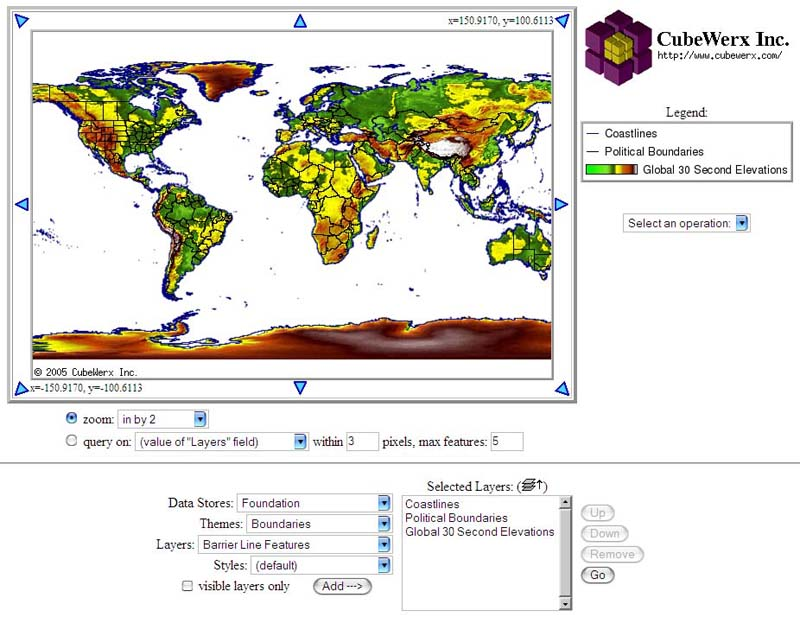
\includegraphics[width=0.90\textwidth]{images/cubewerx.jpg}}
		\caption{CubeXPLOR Demo by CubeWerx Inc.}
	\label{fig:cubewerx}	
\end{figure}
\begin{figure}[h]
		\centering
			\framebox{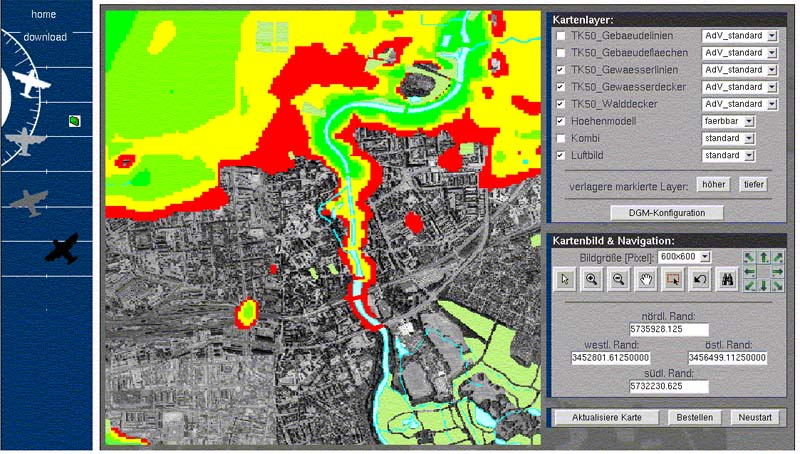
\includegraphics[width=0.90\textwidth]{images/brandenburg.jpg}}
			\caption{Brandenburg WMS - RasGeo Interface}
		\label{fig:brandenburg}
\end{figure}

Even though at their core the two Web Map Services discussed might provide the same capabilities, their user-interfaces and APIs distinguish them in their functionality. Moreover, this functionality is hard-coded and as such these systems cannot dynamically adapt to different user's needs. As it can be observed from Figures \ref{fig:cubewerx} and \ref{fig:brandenburg}, the first noticeable difference is at the language level. Since neither one of the systems provides any description for its terminology and abbreviations, the applications are targeted towards a fixed group of users.

\subsection{Research Approach} \label{subsec:approach}
\indent

As it was shown in Section \ref{subsec:limitations}, the strong interdependence between data representation and its format leads to limitations in terms of application utilities. Since the manipulation of georeferenced data retrieved from various WMSes is of paramount importance in application areas like disaster mitigation, preventing the occurrence of data bottlenecks becomes a top priority.

During the past few years, semantic-based and context-aware techniques have pervaded application areas ranging from science and technology to research and education \cite{mkm2005}. The semantics of an object is determined by its structure (how is the object built up from smaller objects) and its context (what do we already know about these objects, how are they defined, what is their relationship to other objects). As the geodata semantics matches the description above, we have envisioned the development of a knowledge representation and management format, OMGeo, as a solution for separating presentation from structure. However, since we already have an established format for mathematical knowledge, OMDoc, that is both semantic-based and context-aware, we would like to extend it to encompass geosemantics. 

In Section \ref{sec:statement} we will state and analyze the main research problems as they pertain to the development of the OMGeo format, and in Section \ref{sec:strategy} we will detail on the envisioned extension possibility.

%
\section{Statement of the Research Problem} \label{sec:statement}
\indent

As it was shown in the previous sections, the mixture of data format and presentation style considerably reduces the utility of the WMSes. Moreover, since the user-interfaces are hard-coded, clients cannot take full advantage of various WMS applications\footnote{If the user-interface is hard-coded, then the language and the map layers supported are bound to the application in use.} in the absence of nomenclature standards.

Therefore, the overall research problem refers to the separation of the data representation and presentation levels. Furthermore, the data representation level should also encapsulate knowledge about the data in a manner that makes the data content transparent and unambiguous. In the proposed project, we will try to address the following questions:
\begin{enumerate}
	\item Does OMDoc provide a flexible framework to encompass areas of knowledge, other than mathematics?		
	\item Can OMDoc be adapted to encompass geosemantics knowledge?			
	\item How can modularity be achieved so that OMGeo (the extended OMDoc format for georeferenced data) will have an easy way of extending?		
\end{enumerate}

As OMDoc is a semantic-based and context-aware format \cite{kohlhase2004}, we claim that it provides the pillars for the development of OMGeo. Moreover, since the context information for mathematical objects is dynamic and usually both large and highly structured, we assume OMDoc provides a flexible framework to encompass other areas of knowledge \cite{mkm2005}. Since OMDoc was built with a modular concept in mind, extending it involves only the development of additional libraries to capture the geosemantics knowledge. As such, we claim that encompassing geosemantics knowledge can be achieved with minimum adaptation efforts.

As a testing bench for the research claims stated above, the proposed project aims at developing an online demonstrator. In Section \ref{sec:strategy} we will outline the research and development strategy towards the completion of the online demonstrator that will serve as an API to a Web Map Service.

%
\section{Research and Development Strategy} \label{sec:strategy}
\indent

In order to address the research questions and to develop the demonstrator mentioned in Section \ref{sec:statement}, we are planning to carry out the following development steps:
\begin{enumerate}
	\item Extend the OMDoc format to capture geosemantics knowledge.
	\item Develop an OMGeo DTD.
	\item Create sample OMGeo documents.
	\item Develop the API for an example WMS.
\end{enumerate}
The dependence between the above components can be observed in Figure \ref{fig:umlschema}.

Moreover, we will outline each of these components and detail their development process in the next subsections.
\begin{figure}[h]
	\centering		
		\framebox{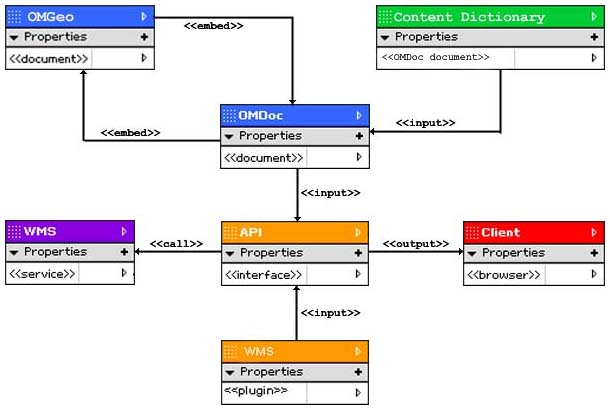
\includegraphics[width=0.90\textwidth]{images/umlschema.jpg}}
		\caption{Module Dependency Schema}
	\label{fig:umlschema}
\end{figure}

\subsection{Extend the OMDoc format to capture geosemantics} \label{subsec:extension}
\indent

As it was shown in the previous sections, a map of georeferenced data can be abstracted to a modular concept with the map layers as the constituent modules. In order to develop a geosemantics format that will overcome the mixture of appearance and structure, we will directly relate to the aforementioned property.

Apart from map data, another area of knowledge where appearance and structure form two distinct entities is mathematics \cite{openmath2004}. The OMDoc format is an open markup language for mathematical documents and more generally the knowledge encapsulated in them in a manner that makes their context and content transparent and unambiguous \cite{kohlhase2004}. It approaches this goal by attaching information to mathematical documents that identify the document structure, the meaning of text fragments, and their relation to other mathematical knowledge in a process called \textit{document markup}. As modular design is generally accepted as best practice in the development of any type of complex application, OMDoc format (version 1.2) also features a modularized language approach. To encompass knowledge, OMDoc makes use of a certain type of libraries called \textit{Content Dictionaries} \cite{kohlhase2004}. A Content Dictionary acts as a container for sets of symbol declarations and knowledge about them, and marks them by \textbf{theory} elements. As such, the OMDoc format becomes easily extensible since the provision of knowledge through Content Dictionaries can make the format applicable to other areas, apart from mathematics. Therefore, in order to encapsulate geodata knowledge, the proposed project aims at developing a number of Content Dictionaries that will refer to the different constituent blocks of a map.

As the content of the \textit{Content Dictionaries} is highly specialized, this project will require a transdisciplinary approach with input from the geoscience field. In order to achieve a better design and better content information, we will cooperate with Prof. Dr. Vikram Unitham from International University Bremen.

\subsection{Develop an OMGeo DTD} \label{subsec:dtd}
\indent

As it was shown in subsection \ref{subsec:extension}, the proposed project aims at developing an extension to OMDoc to include geosemantics knowledge. In order to specify how the geodata should be encapsulated in an OMDoc document, a DTD extension should be attached to the present OMDoc DTD. Even though the RelaxNG\footnote{See http://www.relaxng.org for more information.} method is slowly replacing the DTD and Schema specifications, an OMGeo DTD extension will still be provided. The elements to be defined by the DTD are as yet to be clarified, and will be one of the project results.

\subsection{Create sample OMGeo documents} \label{subsec:sample}
\indent

Upon the creation of valid Content Dictionaries that encapsulate geodata knowledge, documents of OMGeo papers can be written. A case study on sample OMGeo documents will be conducted to test the format's capabilities. Moreover, these documents will also be used as an input to the online demonstrator.

\subsection{Develop the API for an example WMS} \label{subsec:demonstrator}
\indent

Having set up the basis to develop OMGeo documents that are both human and machine understandable, the proposed project will be concluded with an online demonstration of how these documents can interact with a given Web Map Service. For this purpose, an application programming interface will be developed. This API will be developed using J2EE\footnote{See Section \ref{sec:development} for further explanations.} technology and will basically perform the following tasks:
\begin{enumerate}
	\item Receive a plugin\footnote{The plugin will be an XML file where the OMGeo elements will be mapped to WMS specific keywords that are used to query the database.} that will contain the definitions for a specific Web Map Service.
	\item Receive an OMGeo document.
	\item Dynamically transform the OMGeo document into a user-interface.
	\item Use the knowledge encapsulated in the OMGeo document to query the WMS database.
	\item Display the requested map from the Web Map Service.
\end{enumerate}
The module dependency schema in Figure \ref{fig:umlschema} provides a visual representation of the above modules.

%
\section{Development Framework} \label{sec:development}
\indent

As the proposed project considers the development of an online demonstrator as a testing bench, we will outline in this section the software development framework. In particular, we will address the environment and tools that will be used throughout the project. As a conclusion of the section, a reference guide to the expected results will be proposed.

\subsection{Environment and Tools} \label{subsec:tools}
\indent

As the development of the online demonstrator involves querying a Web Map Service, we will make use of the Brandenburg WMS. Since this service is restricted to academic use, it is not publicly available at a specific URL. Therefore, we will make a local installation on a CLAMV\footnote{\textit{CLAMV} stands for \textit{Computational Laboratory for Analysis, Modeling, and Visualization}. More info at http://www.clamv.iu-bremen.de} station. As such a PostgreSQL\footnote{See http://www.postgresql.org for more information.}/Rasdaman\footnote{See http://www.rasdaman.com for more information.} database will be installed on top of a Tomcat server. For the API development, we will use the Java 2 Platform, Enterprise Edition\footnote{J2EE defines the standard for developing component-based multitier enterprise application, featuring Web services support and development tools.} (J2EE). In particular, we will use the Java servlets and Java Server Pages (JSP) technologies. Since the software application will be developed under Linux, we will configure the Emacs editor as a Java IDE (Integrated Development Environment) by installing the Java Development Environment (JDE) for Emacs\footnote{See http://www-106.ibm.com/developerworks/library/j-emacs/?n-j-5241 for more information.}.

\subsection{Expected Results} \label{subsec:results}
\indent

As a suitable evaluation criterion, we would define this project to be successful upon the completion of a running version of the online demonstrator. Since this software application relies on several input modules, we regard the completion of the plugin for the Brandenburg WMS and the creation of the Content Dictionaries for the geosemantics knowledge as important milestones in the overall development. However, as the geosemantics standard behind a georeferenced map does not exist in a unified model, we will not regard our Content Dictionaries to be exhaustive. In the following sections, we will briefly outline a timeline for the proposed project.

%
\section{Schedule of Activities} \label{sec:schedule}
\indent

The activities listed below relate to the Gantt chart in Figure \ref{fig:timeline} that briefly outlines a timeline for the proposed project.
\begin{enumerate}
	\item Develop OMDoc Content Dictionaries to capture geosemantics knowledge.
	\item Develop the OMGeo DTD as an extension of the OMDoc DTD.
	\item Create sample OMGeo documents.
	\item Develop the API WMS plugin for the Brandenburg WMS.
	\item Develop the API for the Brandenburg WMS.
	\item Develop the website that will incorporate the API.
	\item Conduct testing sessions on sample OMGeo documents.
\end{enumerate}
\begin{figure}[h]
	\centering		
		\framebox{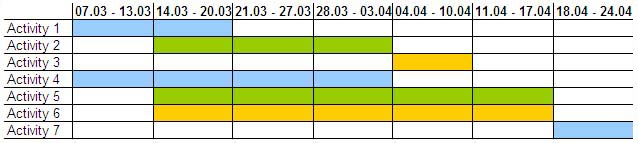
\includegraphics[width=0.90\textwidth]{images/timeline.jpg}}
		\caption{Schedule of Activities}
	\label{fig:timeline}
\end{figure}

Moreover, we will provide a Final Report of the proposed project on April 25, 2005 and will orally present our results in the beginning of May 2005 at International University Bremen.
%
\newpage
%%%%%%%%%%%%%%%%%%%%%%%%%%%%%%%%%%%%%%%%%%%%%%%%%%%%%%%%%%%%%%%%%%
%                                                                %
%                                                                %
%                     The Bibliography                           %
%                                                                %
%                                                                %
%%%%%%%%%%%%%%%%%%%%%%%%%%%%%%%%%%%%%%%%%%%%%%%%%%%%%%%%%%%%%%%%%%

\begin{thebibliography}{0}
%
\bibitem{kohlhase2004}
Kohlhase, M. (2004). OMDoc - An Open Markup Format for Mathematical 
Documents (version 1.2) \textit{http://www.mathweb.org/omdoc/omdoc.ps}, manuscript.
%
\bibitem{kohlhasedtd}
Kohlhase, M. (2004). The OMDoc Document Type Definition \textit{http://www.mathweb.org/omdoc/dtd/omdoc.dtd}.
%
\bibitem{ogc}
de la Beaujardiere, J. (2002). Web Map Service Implementation Specification (version 1.1.1) \textit{Open GIS Consortium Implementation Specification}.
%
\bibitem{openmath2004}
Buswell, S. Caprotti, O. Carlisle, D.P. Dewar, M.C. Gaetano, M. Kohlhase, M. (2004). The OpenMath Standard (version 2.0) \textit{The OpenMath Society}.
%
\bibitem{mkm2005}
Kohlhase, M. (2005). Mathematical Knowledge Management Network of Excellence (version 2.0) \textit{Proposal draft}.
%
\end{thebibliography}

\end{document}
